\documentclass[12pt,letter]{article}

%% \usepackage[fleqn]{amsmath}
\usepackage[margin=1in]{geometry}
\usepackage{amsmath,amsfonts,amsthm,bm}
\usepackage{breqn}
\usepackage{amsmath}
\usepackage{amssymb}
\usepackage{tikz}
\usepackage{algorithm2e}
\usepackage{siunitx}
\usepackage{graphicx}
\usepackage{subcaption}
%% \usepackage{datetime}
\usepackage{multirow}
\usepackage{multicol}
\usepackage{mathrsfs}
\usepackage{fancyhdr}
\usepackage{fancyvrb}
\usepackage{parskip} %turns off paragraph indent
\pagestyle{fancy}

\usetikzlibrary{arrows}

\DeclareMathOperator*{\argmin}{argmin}
\newcommand*{\argminl}{\argmin\limits}

\newcommand{\mathleft}{\@fleqntrue\@mathmargin0pt}
\newcommand{\R}{\mathbb{R}}
\newcommand{\Z}{\mathbb{Z}}
\newcommand{\N}{\mathbb{N}}
\newcommand{\indep}{\perp \!\!\! \perp}

\setcounter{MaxMatrixCols}{20}

\usepackage{listings}

\begin{document}

\rhead{(Bill)Yuan Liu, student \#: 996954078\\ Date: 2020/01/15}
\lhead{CSC2306 - Assignment 0}

\section{Probability}
\subsection{Variance and Covariance}
\begin{enumerate}
\item Starting from the definition of independence, show that the independence of $X$ and $Y$ implies that their covariance is $0$.
  \begin{align*}
    Cov(X,Y)&=E[(X-E[X])(Y-E[Y])]\\
            &=E[XY-YE[X]-YE[X]+E[X]E[Y]]\\
            &=E[XY]-E[Y]E[X]-E[Y]E[X]+E[X]E[Y]\\
            &=E[XY]-E[Y]E[X]\\
    X,Y & \text{ are independent} \implies\\
            & P(X|Y)=P(X)\\
            & P(X,Y)=P(Y)P(X|Y)= P(Y)P(X)\\
    E[XY] &= \int_x \int_y xy p(x,y) dxdy\\
            &= \int_x \int_y xy p(y)p(x|y) dxdy\\
            &= \int_x \int_y xy p(y)p(x) dxdy\\
            &= \int_x x p(x) dx \int_y y p(y) dy\\
    E[X]E[Y] &= \int_x xp(x) dx \int_y yp(y) dy\\
    Cov(X,Y)&=0\\
  \end{align*}

  \pagebreak
  
\item For a scalar constant $a$, show the following two properties starting from the definition of expectation
  \begin{align}
    \mathbb{E}(X+aY) &= \mathbb{E}(X) + a\mathbb{E}(Y)\\
    \text{var}(X + aY) &= \text{var}(X) + a^2 \text{var}(Y)
  \end{align}
  \begin{itemize}    
  \item $\mathbb{E}(X+aY) = \mathbb{E}(X) + a\mathbb{E}(Y)$
      \begin{align*}
        E(X+aY)&=\int_x \int_y p(x,y)(x+ay) dxdy\\
               &=\int_x \int_y p(x)p(y)(x+ay) dxdy\\
               &=\int_x \int_y xp(x,y) + ay p(x,y) dxdy\\
               &=\int_x \int_y xp(x,y) dxdy + \int_x \int_y ay p(x,y) dxdy\\
               &=\int_x xp(x) \int_y p(y) dy dx + \int_y ay p(y) \int_x  p(x) dx dy\\
               &=\int_x xp(x) dx + \int_y ay p(y) dy\\
               &=E[X] + a E[Y]\\
      \end{align*}
    \item $\text{var}(X + aY) = \text{var}(X) + a^2 \text{var}(Y)$
      \begin{align*}
        var(aY)&= \int_y p(y)(ay-E[aY])^2 dy\\
               &= \int_y p(y)(a^2y^2 - 2ayE[aY] + E[aY]^2) dy\\
               &= \int_y p(y)a^2y^2dy - \int_y p(y)2ayE[aY] dy + \int_y p(y)E[aY]^2 dy\\
               &= a^2E[Y^2] - 2a^2E[Y]^2 + a^2 E[Y]^2\\
               &= a^2E[Y^2] - a^2E[Y]^2\\
        var(X+aY)&= E[(X+aY)^2]-E[(X+aY)]^2\\
               &= E[X^2+2aXY+a^2Y^2]-(E[X]+aE[Y])^2\\
               &= E[X^2]+2aE[XY]+a^2E[Y^2]-(E[X]^2+2aE[X]E[Y]+a^2E[Y]^2)\\
               &\text{ from question 1: } X \indep Y \implies E[XY] = E[X]E[Y]\\
               &= E[X^2]+2aE[X]E[Y]+a^2E[Y^2]-(E[X]^2+2aE[X]E[Y]+a^2E[Y]^2)\\
               &= E[X^2]-E[X]^2+a^2E[Y^2]-a^2E[Y]^2\\
               &= var(X)+a^2var(Y)\\
      \end{align*}      
  \end{itemize}
\end{enumerate}

\subsection{1D Gaussian Densities}

\begin{enumerate}
\item Can a probability density function (pdf) ever take values greater than $1$?\\
  
  Yes it is possible as long as the integral adds up to 1 and is non-negative, since the support interval corresponding to values greater than 1 can be made arbitrarily small.\\
  
  \item Let $X$ be a univariate random variable distributed according to a Gaussian distribution with mean $\mu$ and variance $\sigma^2$.

    Write the expression for the pdf:\\

    $f(x) = \frac{1}{\sqrt 2\pi\sigma^2} e^{\frac{(x-\mu)^2}{2\sigma^2}}$\\

    Write the code for the function that computes the pdf at $x$ with default values $\mu=0$ and $\sigma = \sqrt{0.01}$:\\

\begin{verbatim}
function gaussian_pdf(x; mean=0., variance=0.01)
    1. / ((2 * pi * variance)^0.5) * exp(-(x - mean)^2 / (2 * variance))
end
\end{verbatim}

    Test your implementation against a standard implementation from a library:
    
\begin{verbatim}
x = randn()
@test gaussian_pdf(x) ≈ pdf.(Normal(0.,sqrt(0.01)),x)
@test isapprox(gaussian_pdf(x,mean=10., variance=1), 
    pdf.(Normal(10., sqrt(1)),x))
\end{verbatim}

    \item What is the value of the pdf at $x=0$? What is probability that $x=0$ (hint: is this the same as the pdf? Briefly explain your answer.)

      $f(0)=\frac{1}{\sqrt{2 \pi \sigma^2}} \approx 3.9894$\\
      $prob(x=0)=\int_{x=0}^{0}p(x)f(x) dx = 0$ since it is a continuous distribution and probability is the integration over some support. Any integration over an empty interval is 0.\\

    \item A Gaussian with mean $\mu$ and variance $\sigma^2$ can be written as a simple transformation of the standard Gaussian with mean $0.$ and variance $1.$.

      Write the transformation that takes $x \sim \mathcal{N}(0.,1.)$ to $z \sim \mathcal{N}(\mu, \sigma^2)$:\\
      Given $E[X]=0$, $var(X)=1$, then\\
      $E(\sigma X+\mu) = \sigma E(X)+\mu = \mu$\\
      $var(\sigma X+\mu) = \sigma^2 var(X) + 0 = \sigma^2$\\
      so the transformation $\sigma X + \mu$ is valid\\

      Write a code implementation to produce $n$ independent samples from $\mathcal{N}(\mu, \sigma^2)$ by transforming $n$ samples from $\mathcal{N}(0.,1.)$.
\begin{lstlisting}[
    mathescape,
    columns=fullflexible,
    basicstyle=\ttfamily\footnotesize,breaklines=true
    ]
function sample_gaussian(n; mean=0., variance=0.01)
    # from Normal(0,1):
    x = randn(n)
    sqrt(variance).*x .+ mean

    # alternatively using central limit theorem:
    #N(0,1) = $1/m \sum_i(x_i-\mu)/\sqrt{m \sigma^2}$
    #ys = zeros(n)
    #m = 100
    ##X_i from uniform(0,1):
    ##uniform_variance = 1/12.*(1-0)^2=1/12.
    ##uniform_mean = 0.5
    ##N(0,1) = $\sqrt{12/m}\sum_i x_i  - (0.5)\sqrt{12m}$
    #for i=1:n
    #    xs = rand(Float64,m)
    #    ys[i] = sqrt(12. / m) * sum(xs) - sqrt(12. * m)*0.5
    #end;
    #sqrt(variance).*ys.+mean
end;
\end{lstlisting}
      
      Test your implementation by computing statistics on the samples:
\begin{verbatim}
using Statistics: mean, var
@testset "Numerically testing Gaussian Sample Statistics" begin
    samples = sample_gaussian(100000, mean=5., variance=3.5);
    m = mean(samples)
    v = var(samples)
    @test isapprox(m, 5, atol=1e-2)
    @test isapprox(v, 3.5, atol=1e-2)
end;
\end{verbatim}

      \pagebreak
      
    \item Sample $10000$ samples from a Gaussian with mean $10.$ an variance $2$. Plot the **normalized** `histogram` of these samples. On the same axes plot the pdf of this distribution.
Confirm that the histogram approximates the pdf.

\begin{verbatim}
using Plots

samples = sample_gaussian(100000, mean=10., variance=2.);

histogram(samples,normalize=true, 
    label="100000 outputs from sample_gaussian()",
    legend = :bottomright)
    
dist = x -> pdf(Normal(10.,sqrt(2.)),x)
plot!(dist, 2, 18, 
    label="pdf of normal distribution",
    title="Gaussian Sampler Distribution Check (mu=10,sigma^2=2)",
    xlabel="x",
    ylabel="pdf(x), histogram fraction",
    linewidth = 2,
    linecolor = :red)

savefig("sample_gaussian_pdf.png")
\end{verbatim}
\begin{figure}[h]
  \centering
  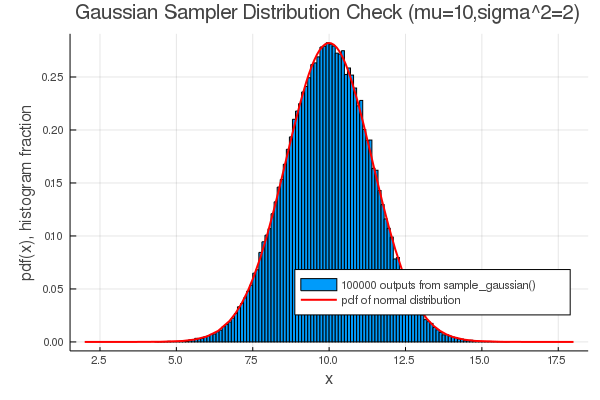
\includegraphics[width=14cm,keepaspectratio]{imgs/sample_gaussian_pdf.png}
\end{figure}
\end{enumerate}

\pagebreak

\section{Calculus}

\subsection{Manual Differentiation}

Let $x,y \in \mathbb{R}^m$, $A \in \mathbb{R}^{m \times n}$, and square matrix $B \in \mathbb{R}^{m \times m}$. And where $x'$ is the transpose of $x$.

\begin{enumerate}
  
\item What is the gradient of $x'y$ with respect to $x$?
  \begin{align*}
    \frac{\partial}{\partial x} x'y &= \frac{\partial}{\partial x} \sum_i x_i y_i\\
    \frac{\partial}{\partial x_j} x'y &= \frac{\partial}{\partial x_j} \sum_i x_i y_i, j =0,..m-1\\
                                    &= \sum_i 1_{j=i}(i)y_i, j =0,..m-1\\
                                    &= y_j, j =0,..m-1\\
    \frac{\partial}{\partial x} x'y &= y\\
  \end{align*}

\item What is the gradient of $x'x$ with respect to $x$?
  \begin{align*}
    \frac{\partial}{\partial x} x'x &= \frac{\partial}{\partial x} \sum_i x_i x_i\\
    \frac{\partial}{\partial x_j} x'x &= \frac{\partial}{\partial x_j} \sum_i x_i x_i, j =0,..m-1\\
                                    &= \sum_i 1_{j=i}(i)2x_i, j =0,..m-1\\
                                    &= 2x_j, j =0,..m-1\\
    \frac{\partial}{\partial x} x'x &= 2x\\
  \end{align*}
\item What is the Jacobian of $x'A$ with respect to $x$?
  \begin{align*}
    \frac{\partial}{\partial x} (x'A)_j &= \frac{\partial}{\partial x} \sum_i a_{ij} x_i, j =0,..,n-1\\
    \frac{\partial}{\partial x_k} (x'A)_j &= \frac{\partial}{\partial x_k} \sum_i a_{ij} x_i, j =0,..,n-1, k=0,..,m-1\\
                                        &= \sum_i 1_{k=i}(i) a_{ij}, j =0,..,n-1, k=0,..,m-1\\
                                        &= a_{kj}, j =0,.,n-1, ,k=0,..,m-1\\
    \frac{\partial}{\partial x_k} (x'A)_j &= a_{kj}, j =0,.,n-1, k=0,..,m-1\\
    \frac{\partial}{\partial x} (x'A) &= A^T\\
  \end{align*}
\item What is the gradient of $x'Bx$ with respect to $x$?
  \begin{align*}
    \frac{\partial}{\partial x_k} (x'Bx)&= \frac{\partial}{\partial x_k}(\sum_i x_i (\sum_j b_{ij}x_j)), k=0,..,m-1\\
                                        &= \sum_i \frac{\partial}{\partial x_k}(x_i) (\sum_j b_{ij}x_j) + \sum_i x_i (\frac{\partial}{\partial x_k}(\sum_j b_{ij}x_j)), k =0,..,m-1\\
                                        &= \sum_i 1_{k=i}(i) (\sum_j b_{ij}x_j) + \sum_i x_i (\sum_j 1_{k=j}(j)b_{ij}), k =0,..,m-1\\
                                        &= \sum_j b_{kj}x_j + \sum_i x_i b_{ik}, k =0,..,m-1\\
    \frac{\partial}{\partial x} (x'Bx)&= Bx + B^Tx
  \end{align*}
\end{enumerate}

\subsection{Automatic Differentiation (AD)}

Use one of the accepted AD library (Zygote.jl (julia), JAX (python), PyTorch (python))
to implement and test your answers above.

\subsubsection{Create Toy Data}
\begin{verbatim}
using LinearAlgebra;
# Choose dimensions of toy data
m = 8
n = 11

x = rand(m,)
y = rand(m,)
A = rand(m,n)
B = rand(m,m)
\end{verbatim}

Test to confirm that the sizes of your data is what you expect:
\begin{verbatim}
@testset "Sizes of Toy Data" begin
    @test (m,) == size(x)
    @test (m,) == size(y)
    @test (m,n) == size(A)
    @test (m,m) == size(B)
end;
\end{verbatim}

\subsubsection{Automatic Differentiation}

\begin{enumerate}
  \item Compute the gradient of $f_1(x) = x'y$ with respect to $x$?

\begin{verbatim}
using Zygote;
    g1 = gradient((x, y) -> x' * y, x, y)[1];
\end{verbatim}

  \item Compute the gradient of $f_2(x) = x'x$ with respect to $x$?
\begin{verbatim}
    g2 = gradient(x-> x' * x, x)[1];
\end{verbatim}

  \item Compute the Jacobian of $f_3(x) = x'A$ with respect to $x$?
\begin{verbatim}
    g3 = zeros(n,m);
    for i=1:size(A)[2] #1 to n
        g3[i,:] = gradient((x, A) -> (x' * A)[i], x, A)[1]
    end;
\end{verbatim}

    \pagebreak
    
    Briefly, explain why `gradient` of $f_3$ is not well defined (hint: what is the dimensionality of the output?) and what the `jacobian` function is doing in terms of calls to `gradient`.\\

    Output of $f_3$ is a high dimensional object and gradient of reverse mode is computable for pairs of input-output given fixed output. Thus it cannot compute the Jacobian in one reverse mode pass since it can only compute one directional derivative starting at the output while the Jacobian requires isolation of each components of the output in order to compute pairwise sensitivies of each ouput component with respect to each input.\\
    
    The autodiff package is doing reverse mode by traversing adjoint graph that is constructable (such as using graph transformations) on the forward pass and computing sensitivities with respect to the output on the backward pass using builtin or user provided adjoint for each involved operation. In the case of multidimensional output, the reverse mode has to be propagated for each of the dimensions of the output, where in each pass sensitives are computed from the selected output scalar towards the leaves (eg: input variables). These frameworks (reverse and forward) are implementable using vector jacobian products and dual numbers.\\
    
    Specifically, how many calls of `gradient` is required to compute a whole `jacobian` for $f : \mathbb{R}^m \rightarrow \mathbb{R}^n$?\\

    n calls to gradient function are needed where each call has complexity of the reverse adjoint graph that it traverses through.\\

\item Compute the gradient of $f_4(x) = x'Bx$ with respect to $x$?
\begin{verbatim}
    g4 = gradient((x, B) -> x' * B * x, x, B)[1];
\end{verbatim}

\item Test all your implementations against the manually derived derivatives in previous question

  \begin{lstlisting}[
    mathescape,
    columns=fullflexible,
    basicstyle=\ttfamily\footnotesize,breaklines=true
    ]
    @test g1 $\approx$ y
    @test g2 $\approx$ 2 * x
    @test g3 $\approx$ A'
    @test g4 $\approx$ B*x + B'*x
  \end{lstlisting}

\end{enumerate}

\pagebreak

\section{Appendix}

Entire code (A0\_code.jl) for the assignment is shown here.
  \begin{lstlisting}[
    mathescape,
    columns=fullflexible,
    basicstyle=\ttfamily\footnotesize,breaklines=true
    ]
using Test
using Distributions

function gaussian_pdf(x; mean=0., variance=0.01)
    1. / ((2 * pi * variance)^0.5) * exp(-(x - mean)^2 / (2 * variance))
end;

x = randn()
@test gaussian_pdf(x) ≈ pdf.(Normal(0.,sqrt(0.01)),x)
@test isapprox(gaussian_pdf(x,mean=10., variance=1) ,
    pdf.(Normal(10., sqrt(1)),x))

function sample_gaussian(n; mean=0., variance=0.01)
    # from Normal(0,1):
    x = randn(n)
    sqrt(variance).* x .+ mean

    # #alternatively using central limit theorem:
    #N(0,1) = $1/m \sum_i(x_i-\mu)/\sqrt{m \sigma^2}$
    # ys = zeros(n)
    # m = 100
    # #X_i from uniform(0,1):
    # #uniform_variance = 1/12.*(1-0)^2=1/12.
    # #uniform_mean = 0.5
    # #N(0,1) = $sqrt(12/m)\sum_i(x_i) - sqrt(12m)(0.5)$
    # for i=1:n
    #     xs = rand(Float64,m)
    #     ys[i] = sqrt(12. / m) * sum(xs) - sqrt(12. * m)*0.5
    # end;
    # sqrt(variance).*ys.+mean
end;

using Statistics: mean, var
@testset "Numerically testing Gaussian Sample Statistics" begin
    samples = sample_gaussian(100000, mean=5., variance=3.5);
    m = mean(samples)
    v = var(samples)
    @test isapprox(m, 5, atol=1e-2)
    @test isapprox(v, 3.5, atol=1e-2)
end;

samples = sample_gaussian(100000, mean=10., variance=2.);

using Plots

histogram(samples,normalize=true,
    label="100000 outputs from sample_gaussian()",
    legend = :bottomright)

dist = x -> pdf(Normal(10.,sqrt(2.)),x)
plot!(dist, 2, 18,
    label="pdf of normal distribution",
    title="Gaussian Sampler Distribution Check (mu=10,sigma^2=2)",
    xlabel="x",
    ylabel="pdf(x), histogram fraction",
    linewidth = 2,
    linecolor = :red)

savefig("sample_gaussian_pdf.png")

using LinearAlgebra;
# Choose dimensions of toy data
m = 8
n = 11

x = rand(m,)
y = rand(m,)
A = rand(m,n)
B = rand(m,m)

# Make sure your toy data is the size you expect!
@testset "Sizes of Toy Data" begin
    @test (m,) == size(x)
    @test (m,) == size(y)
    @test (m,n) == size(A)
    @test (m,m) == size(B)
end;

using Zygote;

@testset "derivative checks" begin
    g1 = gradient((x, y) -> x' * y, x, y)[1];
    g2 = gradient(x-> x' * x, x)[1];
    g3 = zeros(n,m);
    for i=1:size(A)[2] #1 to n
        g3[i,:] = gradient((x, A) -> (x' * A)[i], x, A)[1]
    end;
    g4 = gradient((x, B) -> x' * B * x, x, B)[1];
    @test g1 $\approx$ y
    @test g2 $\approx$ 2 * x
    @test g3 $\approx$ A'
    @test g4 $\approx$ B*x + B'*x
end;

  \end{lstlisting}

\end{document}